\documentclass[class=article, crop=false]{standalone}

\begin{document}

The type of motion artifact and its severity depends on the magnitude and type of motion, as well as its temporal relation to the pulse sequence. This makes a general description of motion effects quite difficult, as the same type of motion may have different effects across scans. In the following discussion, a broad distinction will be made between \textit{inter-shot} and \textit{intra-shot} effects (Fig. \ref{fig:fig1}). Inter-shot effects are the result of movement during the latent periods in the scan between data acquisition and the following excitation (or shot). For motion that occurs between shots and data acquisition, intra-view effects will be present.

\begin{figure}[h]
	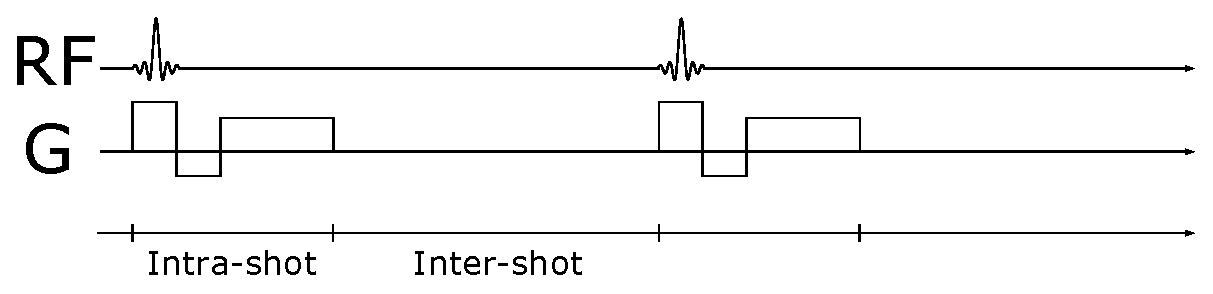
\includegraphics[scale=0.7]{Fig1}
	\centering
	\caption{During an MRI scan, motion can be classified as happening 'intra-shot' or 'inter-shot'. Intra-shot motion is motion that occurs between RF excitation and data acquisition. The inter-shot time interval is the period of time between excitation pulses when gradients are not switched on, and data is not being encoded or acquired.}
	\label{fig:fig1}
\end{figure}

\subsection{Inter-shot Effects}

For many MR sequences, the intra-shot time interval is much smaller than the repetition time, as well as the characteristic time-scales of \textit{in vivo} motion. In this case, it can be assumed that no motion occurs during this period. Rather, the spin density is essentially displaced from one excitation to the next, that is, during the `inter-shot' period. For inter-shot effects, we will be mainly discussing bulk motion, which is the movement of large structures within the image, or the entire field of view itself. 
\par
Perhaps the most obvious sign that motion has occurred during a scan is the presence of blurring and ghosts in the reconstructed image. Blurring is the smearing of edges, while ghosting is the presence of repeated structures. Both of these artifacts can arise due to inconsistencies in k-space caused by bulk motion. Following the approach of Zahneisen and Ernst \parencite*{Zahneisen2016}, a homogeneous coordinate formalism will be used to analyse acquired k-space when motion is present.

\subsubsection*{Homogeneous Representation of Bulk Motion}
Homogeneous coordinates are widely used in computer vision, and allow for the concise representation of projective, affine and rigid body transformations. A point in three dimensional space $\textbf{r}_0 = \begin{bmatrix} x,&y,&z\end{bmatrix}^{T}$ is represented in homogeneous coordinates by the augmented vector $\tilde{\textbf{r}}_0 = \begin{bmatrix}x,&y,&z,&1\end{bmatrix}^{T}$. This augmented vector can then be operated on by a $4\times4$ homogeneous matrix \textbf{A}.
\begin{equation}
	\label{eq1}
	\tilde{\textbf{r}} = \textbf{A}\tilde{\textbf{r}}_0
\end{equation}
For our purposes, \textbf{A} represents either a rigid body (rotations and translations only) or affine (shearing, scaling, as well as rigid body) transformation. Rigid body motion is characterised by six degrees of freedom (three for translation, and three for rotation). The homogeneous matrix representation of this type of motion can be written as $\textbf{A} = \begin{bmatrix} \textbf{R} & \textbf{d} \\ \textbf{0} & 1 \end{bmatrix}$, where \textbf{R} is $3\times3$ rotation matrix and \textbf{d} is a $3\times1$ translation vector. It can thus be verified that Eq. (\ref{eq1}) is the homogeneous representation of $\textbf{r} = \textbf{R} \textbf{r}_0 + \textbf{d}$.
\par
Affinities are a higher order group of transformations than rigid body transforms, and require twelve degrees of freedom to characterise. They can also be represented as a $4\times4$ matrix \textbf{A}, but with the $3\times3$ matrix \textbf{R} from the rigid body case replaced with a matrix \textbf{S}, which has the same dimensions. \textbf{S} contains not only the parameters that describe rotation, but also shearing and scaling.
\par
\textit{In vivo} motion can be quite complex, such that time-dependent deformation fields would be needed for its full characterisation. In practice however, this complete description is often not necessary, and a simplified model is sufficient. For example, respiratory movement is often modelled as periodic motion in one dimension. Rigid body transformations are used to model head motion in neural imaging \parencite{Godenschweger2016}, and affine (as well as rigid body) models have been used to describe motion in cardiac and abdominal imaging \parencite{Henningsson2014,Nehrke2005,Manke2002}. While affine models of \textit{in vivo} motion are quite useful, it is important to keep in mind that they are only a useful local approximation for a region of interest, and generally not applicable to the entire field of view.
\par
Nevertheless, in the following investigation we will assume that the points or voxels $\tilde{\textbf{r}}_0$ in the imaging volume are undergoing motion that can be modelled as an affine transformation. The movement of $\tilde{\textbf{r}}_0$ to a new position $\tilde{\textbf{r}}$ can therefore be described by Eq. (\ref{eq1}).

\subsubsection*{Motion and K-space Inconsistencies}

Acquired signal in MRI can be written as
\begin{equation}
	\label{eq2}
	s(\tilde{\textbf{k}}) = \int d\textbf{V} \rho\left(\tilde{\textbf{r}}\right)\operatorname{e}^{-i2\pi\tilde{\textbf{r}}^{T}\tilde{\textbf{k}}}
\end{equation}
where $\tilde{\textbf{r}}$ and $\tilde{\textbf{k}}$ are homogeneous coordinate vectors. The vector $\tilde{\textbf{k}} = \begin{bmatrix}k_{x},&k_{y},&k_{z},&\varphi\end{bmatrix}^{T}$, with $\varphi$ representing an initial phase.
\par
Let $\tilde{\textbf{r}}_0$ and $\tilde{\textbf{k}}_0$ represent the augmented, position and k-space vectors when no motion is present. Now assume that some movement occurs, such that $\tilde{\textbf{r}}_0$ is transformed to $\tilde{\textbf{r}}$ by the affine matrix \textbf{A}. The phase factor in Eq. (\ref{eq2}) which we call $\Phi$ is therefore
\begin{equation} \label{eq3}
	\begin{split}
		\Phi & = \tilde{\textbf{r}}^T\tilde{\textbf{k}}_0 \\ 
			 & = (\textbf{A}\tilde{\textbf{r}}_0)^T\tilde{\textbf{k}}_0
		     = {\tilde{\textbf{r}}_0}^T\textbf{A}^T\tilde{\textbf{k}}_0 \\
		     & = {\tilde{\textbf{r}}_0}^T\tilde{\textbf{k}}.
	\end{split}
\end{equation}
An interpretation of the above operations is that we are keeping the body reference frame fixed, and rather than sampling the points $\tilde{\textbf{k}}_0$, we are now sampling the coordinates $\tilde{\textbf{k}}$ in a transformed k-space due to motion (Fig 1.). Under the assumption of no motion, the sampled signal values at points $\tilde{\textbf{k}}$ will be incorrectly mapped to $\tilde{\textbf{k}}_0$.  In the case where \textbf{A} is a rigid body transformation with $3\times3$ rotation matrix \textbf{R} and translation vector $\textbf{d} = \begin{bmatrix}\Delta_x,&\Delta_y,&\Delta_z\end{bmatrix}^T$,
\begin{equation} \label{eq4}
	\begin{split}
		\tilde{\textbf{k}} & = \textbf{A}^T\tilde{\textbf{k}}_0
		= \begin{bmatrix}\textbf{R}^T & \textbf{0} \\ \textbf{d}^T & 1\end{bmatrix}\begin{bmatrix}k_{0x}\\k_{0y}\\k_{0z}\\\varphi_0\end{bmatrix}\\
		& = \begin{bmatrix}k_{x}\\k_{y}\\k_{z}\\\Delta_{x}k_{0x} + \Delta_{y}k_{0y} + \Delta_{z}k_{0z} + \varphi_0\end{bmatrix}.
	\end{split}
\end{equation}
We can see that rigid body motion results in a rotation of the original k-space coordinates by $\textbf{R}^T$, and the addition of a phase term ($\Delta_{x}k_{0x} + \Delta_{y}k_{0y} + \Delta_{z}k_{0z}$) to the initial value $\varphi_0$. Generality under an affine transformation is not lost here, $\textbf{R}^T$ would simply be replaced by $\textbf{S}^T$. The use of homogeneous coordinates therefore allows for the succinct representation of acquired signal when a motion \textbf{A} occurs:
\begin{equation} \label{eq5}
s(\tilde{\textbf{k}}) = \int d\textbf{V} \rho\left(\tilde{\textbf{r}}_0\right)\operatorname{e}^{-i2\pi{\tilde{\textbf{r}}_0}^{T}\textbf{A}^T\tilde{\textbf{k}}_0}.
\end{equation}
\par
K-space acquisition is sequential, rather than instantaneous, and thus the k-space coordinates have an implicit time dependence. The motion is also a function of time, \textbf{A(t)}. Depending on the acquisition trajectory and \textbf{A(t)}, $\tilde{\textbf{k}}$ may be quite displaced from the `motion-free' $\tilde{\textbf{k}}_0$, and signal values at $\tilde{\textbf{k}}$ will have no correspondence with those at $\tilde{\textbf{k}}_0$. If \textbf{A(t)} is unknown or not accounted for, this misregistration of k-space data can cause inconsistencies. For Cartesian k-space trajectories, these inconsistencies occur across lines in the phase encoding direction. Generally speaking, if these displacements are small from line to line, (such as in the case of slow, continuous motion), blurring will be present in the reconstructed image. Frequent, periodic displacements and large rotations can cause periodic phase modulations and large inconsistencies in the k-space data, which results in ghosting.
\par
When k-space data is acquired under the assumption of no motion, correction may be possible, provided the motion \textbf{A(t)} is known. This is done by transforming the points $\tilde{\textbf{k}}_0$ by $\textbf{A(t)}^T$, such that the measured signal value is correctly mapped to position in k-space. Another approach would be to scrap the `no motion' assumption, and update our data collection algorithm in real time. The former method is the principle behind `retrospective motion correction', while the latter approach is `prospective motion correction'. Both of these will be discussed in Section 4.

\subsubsection*{Spin History}
Motion between excitations can have effects other than blurring and ghosting. Spin history artifacts can arise in regions where $TR$ is comparable to or less than $T_1$. In this case, out of plane motion causes regions within the object being scanned to be irradiated non-uniformly. Voxels which may have otherwise identical contrast properties may produce vastly different signals because of their different excitation history. This is due to the longitudinal magnetisation not fully recovering, causing measured signal to vary from excitation to excitation. Spin history effects are especially of concern in fMRI \parencite{Friston1996,Muresan2005}, where brain activation is identified by changes in blood oxygen level dependent (BOLD) signals in the order of 1\%-5\%. Hence even small noise contributions due to motion can lead to false activations. Spin history effects are not corrected by post-processing steps which aim to realign displaced slices and volumes.

\subsubsection*{Field Inhomogeneities}
Magnetic field inhomogeneities are introduced by local variations in magnetic susceptibility \textit{in vivo}.

\subsection{Intra-shot Effects}
In the previous subsection, it was assumed that no movement occurred during the intra-shot period, and so the object was displaced from excitation to excitation. Here, we consider the possibility of motion during the interval between excitation and data acquisition. In other words, spins are moving while gradients are turned on. Intra-shot translations along gradient directions cause well known `flow effects' \parencite{Barth1985}. While this can be the source of contrast in diffusion weighted imaging, additional intra-scan bulk motion is a severe problem in this modality \parencite{LeBihan2006}.
\par
Intra-shot effects can be understood through the concept of gradient moments. Spatial information is encoded in the phase of the precessing magnetization through the use of magnetic field gradients. Phase induced is therefore dependent on position:
\begin{equation} \label{eq6}
	\Phi = \gamma\int^{t}\textbf{r}\textbf{G($\tau$)}d\tau,
\end{equation}
where \textbf{G($\tau$)} is the three dimensional gradient vector at time $\tau$. If there is no intra-shot motion, \textbf{r} has no time dependence and can be taken outside the integral. The other factors in Eq. (\ref{eq6}) define the `zeroth' gradient moment:
\begin{equation} \label{eq7}
	M_0 = \gamma\int^{t}\textbf{G($\tau$)}d\tau.
\end{equation}
Consider now a constant intra-scan translation, described by $\textbf{r} = \textbf{r}_0 + t\textbf{v}$. \textbf{r} is now time dependent and so
\begin{equation} \label{eq8}
	\begin{split}
		\Phi & = \gamma\int^t(\textbf{r}_0 + \tau\textbf{v})\textbf{G($\tau$)}d\tau \\
			 & = \textbf{r}_0\gamma\int^t\textbf{G($\tau$)}d\tau + \textbf{v}\gamma\int^t\tau\textbf{G($\tau$)}d\tau \\
			 & = \textbf{r}_0M_0 + \textbf{v}M_1.
	\end{split}
\end{equation}
$M_1 = \gamma\int^t\tau\textbf{G($\tau$)}d\tau$ is similarly defined as the first gradient moment. Higher order moments are present when more complex motions occur. Intra-scan motion thus results in the addition of a velocity dependent phase.
\par
In traditional spin echo sequences, $M_0$ is set to zero at the echo time, so that the centre of the frequency encoding line is sampled at this point. $M_1$ will not be zero at this point in time however (unless velocity is 0), and a loss of signal due to dephasing will result. Gradient moment nulling or `velocity compensation' is a technique that has been around for some time to try and mitigate this effect \parencite{Haacke1987}. It involves applying additional gradient lobes in the sequence that set $M_0$ as well as $M_1$ to $0$ at echo time. Even so, $M_1$ will not be $0$ away from the centre of k-space, thus flow effects can still be prevalent.
\par
In EPI, nonzero $M_1$ causes ghosting and blurring which is especially pronounced if there is intra-shot motion in the frequency encoding direction. Spiral acquisitions are less susceptible to flow effects, as the sampling trajectory means $M_1$ is quite small near the k-space origin compared to Cartesian sequences \parencite{Irarrazaval1999,Nishimura}. Radial trajectories with projection reconstruction have also been found to be much less susceptible to the effects of flow \parencite{Nishimura1991}.
\par
The problem of intra-shot motion is a difficult one, and quite relevant despite the lack of attention it receives compared to inter-shot motion. While gradient moment nulling is quite effective, the presence of higher order moments, pulsatile flow and the fact that it requires additional time within the pulse sequence means that it is not a wholly effective technique. Most of the interest in mitigating the effects of intra-shot motion is due to the effect it has in diffusion imaging. Many motion correction techniques in this area therefore target both intra-scan and inter-scan motion.

\subsection{Summary}
We have seen how motion causes degradation of quality in MR images. Movement can cause ghosting, blurring, loss of contrast, and artificially strong or weak signals. Depending on the pulse sequence, where the motion occurs and when the motion occurs, the magnitude of these effects may vary.

\end{document}